%!TEX root = ../BoYu-Dissertation.tex
\graphicspath{{Figures/}}

\chapter{Our Approach: Knowledge Representation} % (fold)
\label{cha:knowledge_reprsentation}
We describe the two major knowledge components in this chapter: the computational representation of the field of work, and the events. We first provides a formalization of the field of work using a first-order logic, augmented with several modal operators and meta predicates. The formalization is not intended to be directly implemented, rather it is intended to be used as a specification for designing knowledge representation and reasoning capabilities. We then discuss how the formalization can be computational represented using the PlanGraph model. At last, we discuss the specification and typology of events in our approach.

\section{Formalizing the Field of Work} % (fold)
\label{sec:formalizaing_the_field_of_work}
In general, the field of work in a collaborative activity can be defined as a domain model that includes three related sub-models $FoW=\{ER, LS, DEP\}$: the model of basic entities and their relations $ER$, the set of all actors' local scopes $LS$, and the set of dependencies among activities $DEP$. $ER$ provides the basic vocabulary for defining local scopes $LS$ and dependencies $DEP$. We elaborate on the three components in the rest of this section. 

\subsection{Entities and relations} % (fold)
\label{sub:entities_relations}
\subsubsection{Entities} % (fold)
\label{ssub:entities}
Following the conceptualization of the field of work in Section \ref{sub:the_field_of_work}, 
we define three basic entities that are the basic building blocks in a collaborative activity:
\begin{enumerate}
    \item \textbf{Actors} are defined as human actors participated in a collaborative activity, capable of making decisions and performing actions. $AR=\{ar_1, ar_2, ..., ar_n\}$ is the set of all the actors in a collaborative activity.
    \item \textbf{Resources} are anything that can be used in the transformation process of an activity, including both material resource and resources for thinking. We use $RES=\{res_1, res_2, ..., res_n\}$ to denote the set of resources used in a collaborative activity.
	\item \textbf{Actions} include all the actions that have been performed, is under execution, or will be performed in a collaborative activity. $ACT=\{a_1, a_2, ..., a_n\}$ denotes the set of actions. 
\end{enumerate}

We presume all the basic entities fall into types. Each \emph{action type} represents a class of actions that can be performed by executing a set of subsidiary tasks, commonly called a \emph{recipe}. For example, an actor might rent a car by walking to the rental car center, selecting the car, paying the money, and so forth. Each \emph{resource type} represents a class of resource objects that share the same list of properties and behaviors. For example, every car at the rental car center has a make, model, rental price, etc. Each \emph{actor type} represents a role that abstracts the behaviors of a social actor within some specialized context or domain of endeavor \cite{Bresciani2004}. Its characteristics are easily transferable to other social actors. For example, every actor at the rental car center in the role of `receptionist' can help the customer to rent a car.

We follow Hunsberger and Ortiz \cite{Hunsberger} to use the $@$ constructor to make the distinction between types and instances of entities in the formalization. Each type expression is defined as a unique keyword (e.g. $AType$), then each instance is in the form of the type keyword followed by a set of arguments necessary to identify it (e.g. $AType@arg_1(val_1)@arg_2(val_2)...@arg_n(val_n)$). For example, $drive$ can be an action type and an instance could be $drive@car(car_3)@from(loc_1)@to(loc_2)$ that specifies an instance of driving $car_3$ from location $loc_1$ to $loc_2$. $receptionist@name(Mike)$ is an actor named $Mike$ in the role of $receptionist$. To simplify the expression, we may sometimes use a type keyword followed by a subscript to define an instance. For example, $receptionist_1$ can be used to define an instance of $receptionist$.

% subsubsection entities (end)
\subsubsection{Relations} % (fold)
\label{ssub:relations}
The relations between these entities can be defined using predicate symbols. For example, predicate symbol $Located_in$ can be used to indicate the spatial relation of one entity is inside the second entity. The fact that actor $ar_1$ is in the office $room_3$ can be expressed as $Located_in(ar_1, room_3)$. The list of predicate symbols and their meanings are usually domain dependent. However, here we are more interested in defining a subset of relations between these entities that reflect the common characteristics of activity structure, and are used later to define the local scopes $LS$ and dependencies $DEP$.

\paragraph*{Actor's intention towards action} % (fold)
\label{par:relations_between_action_and_agent}
We follow the SharedPlans theory \cite{grosz1996collaborative} to define three types of intention predicates, $Pot.Int$, $Int.Th$, and $Int.To$, to represent the \emph{intentions} towards an action that have been adopted by an actor. 
\begin{enumerate}
	\item $Pot.Int$ is used to indicate that an actor would like to adopt an intention that the action be performed, but which has not yet be committed to.
	\item $Int.Th$ is used to represent an agent's intention that the action be performed.
	\item $Int.To$ is used to represent an agent's intention to do some action.
\end{enumerate}

 The major difference between these three is the level of commitment the actor has on the action. $Pot.Int(ar_1, act_1)$ indicates that actor $ar_1$ is considering adopting the intention that the action be performed, but has not yet committed to it. $Int.Th(ar_1, act_1)$ indicates that actor $ar_1$ has intended that the action $act_1$ be successfully performed, but it could be performed by other actors. The actor may commit to help the other actors to get it done, or avoid conflicts, but is not participated in the performance of the action. In the proposition $Int.To(ar_1, act_1)$, the actor $ar_1$ has full commitment to perform action $act_1$, i.e. $ar_1$ will participate in the performance of the action $act_1$.

In addition to the three intention predicates, we also define the $Perform$ predicate to indicate that the actor is in the process of performing the action.

% paragraph relations_between_action_and_agent (end)

\paragraph*{Actor's capability of performing action} % (fold)
\label{par:actor_s_capability_of_performing_action}
The \emph{capability} of an actor to perform an action can be defined using three predicates:
\begin{enumerate}
	\item $Knows$ is used to indicate that the actor has the knowledge about how to perform the action, i.e. the actor has at least one recipe to perform the action.
	\item $Able$ indicates that the actor has the ability (e.g. expertise, skills, resources) to perform the action.
	\item $Workable$ indicates that the actor can actually perform the action by satisfying all the constraints and pre-conditions.
\end{enumerate}

The three \emph{capability} predicates describe different levels of capability of an actor on an action. $Knows(ar_1, act_1)$ merely says that $ar_1$ knows how to perform the action $act_1$, but may not be able to perform it. For example, a blind man may know how to drive a car, but do not have the ability to drive it. Furthermore, $Able(ar_1, act_1)$ indicates that the $ar_1$ has the ability to perform the action $act_1$, but it does not necessarily mean the actor can actually perform it. A man who is able to drive the car may be located in a different country, and hence he cannot actually drive it. $Workable(ar_1, act_1)$ defines the highest level of capability, as the $ar_1$ can meet all the constraints and actually perform the action $act_1$.
% paragraph actor_s_capability_of_performing_action (end)

\paragraph*{Relations between actions} % (fold)
\label{par:relations_between_actions}
An important characteristic of actions is that they can be either basic or complex. A \emph{basic} action can be directly executed. A \emph{complex} action, however, cannot be directly executable because it needs to be decomposed into subsidiary actions. The relations between an action and its subsidiary actions can be represented by the predicate $Sub.Act$. $Sub.Act(act_1, act_2)$ indicates that $act_1$ is a subsidiary action of performing $act_2$ within the current plan. The $Sub.Act$ predicate only indicates the relationships between these two actions under the context of current plan. If the plan is changed, the relationship may no longer hold.

Besides the \emph{decomposition} relation between actions, the actions can also be related by the \emph{precedence} relation. The $Precedes)$ relation defines the temporal order of performing two actions at the same level. For instance, $Precedes(act_1, act_2)$ indicates that $act_1$ should be performed before $act_2$. 
% paragraph relations_between_actions (end)

\paragraph*{Relations between action and resource} % (fold)
\label{par:relations_between_action_and_resource}
We use two predicates, $Consumes$ and $Produces$ to define the relations between an action and a resource. $Consumes(act_1, res_1)$ refers to the situation that the performance of action $act_1$ requires the use of resource $res_1$. On the other hand, $Produces(act_1, res_1)$ indicates that action the performance of $act_1$ will produce the resource $res_1$, or make the resource ready for other actions.

\fxerror{add a table to summarize all the relations described in this section.}

% paragraph relations_between_action_and_resource (end)
% subsubsection relations (end)
% subsection entities_relations (end)
\subsection{Local scopes} % (fold)
\label{sub:local_scopes}
We define the local scopes of actors based on two types of relations between actors and actions, i.e. \emph{intention} and \emph{capability}, defined in Section \ref{ssub:relations}. 

\begin{enumerate}
	\item The \emph{intention} relations define the set of actions that an actor has intention or potential intention towards their performance. As we assume the actors' behaviors be goal-driven \cite{nardi1996context}, this set of actions can be used to define the sub-space of the field of work that the actor is willing to work on, we call it \emph{local scope of intention}.
	\item The \emph{capability} relations define the set of actions that the actor have certain level of capability to work on. This set of actions define the sub-space of the field of work that the actor can have impact on, we call it \emph{local scope of capability}.
\end{enumerate}

The whole local scope of work for an user is then defined as the union of these two sub-spaces defined by the \emph{intention} and \emph{capability} relations (Figure \ref{fig:local_scope}). The actions within the intersect of these two sub-spaces are these that the actor actively participate in. The actions within the \emph{local scope of intention}, but outside the \emph{local scope of capability} are these that the actor may need help from other actors. The actions outside the \emph{local scope of intention}, but inside the \emph{local scope of capability} are where the actor can offer help to other actors.

\begin{figure}[htbp] %  figure placement: here, top, bottom, or page
   \centering
   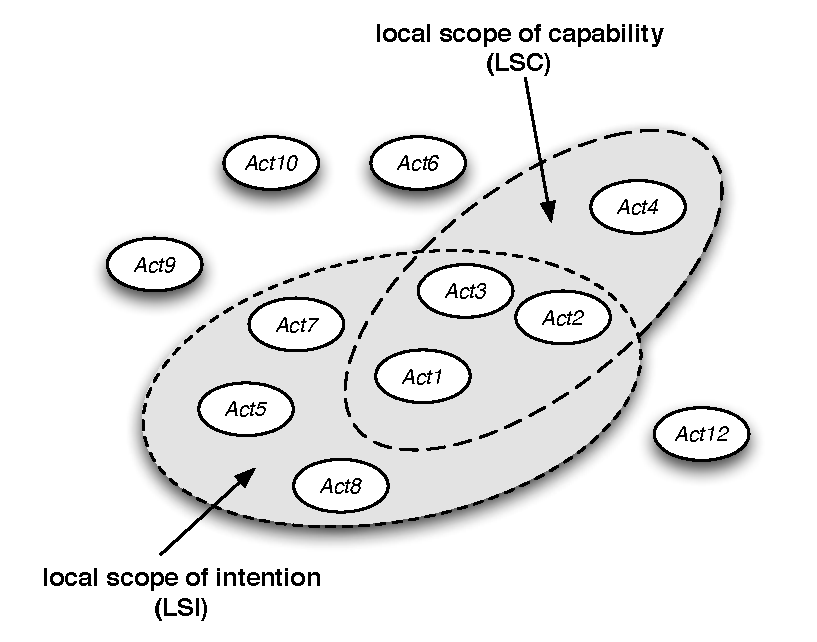
\includegraphics[width=3.5in]{local_scope.pdf} 
   \caption{The structure of local scope of work}
   \label{fig:local_scope}
\end{figure}

One thing to note is that the actions within the same sub-space can have different relations with the actor. That is, the actions in the \emph{local scope of intention} can be either potentially intended ($Pos.Int$), intended that it be performed ($Int.Th$), or intended to be performed ($Int.To$). Similarly, the actions in the \emph{local scope of capability} can also be related to the actor with different levels of capability (i.e. $Knows$, $Able$, $Workable$). As a result, we cannot define the local scope for each actor just as a set of actions, but also with the corresponding relations.

Following this, we define the \emph{local scope of intention} for an actor $LSI(ar)$ as a set of tuples, and each tuple includes three elements: the actor, the action, and the intention relation between them:
\begin{align*} 
	LSI(ar) = \{<ar, act, rel(ar, act)>\}
\end{align*}
where $act\in ACT$ and $rel\in \{Pos.Int, Int.Th, Int.To, Perform\}$.

Similarly, the \emph{local scope of capability} for an actor $LSC(ar)$ is defined as:
\begin{align*} 
	LSC(ar) = \{<ar, act, rel(ar, act)>\}
\end{align*}
where $act\in ACT$ and $rel\in \{Knows, Able, Workable\}$.

Thereafter, the \emph{local scope of work} for an actor $LS(ar)$ is defined as:
\begin{align*} 
	LS(ar) = LSI(ar) \cup LSC(ar)
\end{align*}
% subsection local_scopes (end)
\subsection{Dependencies} % (fold)
\label{sub:dependencies}
We can now focus on the modeling of dependencies between actions. In general, a dependency is defined as a meta-predicate ($DEP$) on two actions ($act_1$, $act_2$) and a proposition $p$, where $act_1$ depends on $act_2$ because of some proposition $p$, and is denoted by $DEP(act_1, act_2, p)$. We follow the terms used in \cite{yu1993actor} to call the depending entity $act_1$ the \emph{depender}, and the entity who is depended upon $act_2$ the \emph{dependee}, and the proposition representing the dependency relation \emph{dependum}.

Based on the various types of relations between actions and resources defined in Section \ref{ssub:relations}, we can use them to define the various types of dependencies described in our conceptual framework in Section \ref{ssub:dependencies}. 

\paragraph*{Temporal dependency} % (fold)
\label{par:temporal_dependencies_}
The predicate $Precedes$ can be used to define the temporal dependency between actions, i.e. the performance of the action $act_2$ as \emph{depender} depends on the performance of the action $act_1$ as \emph{dependee}, because $act_1$ is a pre-requisite action that must have been completed at the time when $a_2$ is performed. $Precedes(act_1, act_2)$ is the \emph{dependum} in this case.
\begin{align*} 
	 DEP(act_2, act_1, Precede(act_1, act_2))
\end{align*}
% paragraph temporal_dependencies_ (end)

\paragraph*{Resource dependencies} % (fold)
\label{par:resource_dependencies}
The predicates $Consumes$ and $Produces$ can be used to define the three types of resource dependencies. 

A \emph{fit dependency} occurs when two actions ($act_1$, $act_2$) collectively produce the same resource ($res_1$). In this case, the two actions  are mutually dependent on each other, i.e. both can be \emph{depender} and \emph{dependee} at the same time. The \emph{dependum} is the combination of two predicates: $Produces(act_1, res_1)$ and $Produces(act_2, res_1)$.
\begin{align*} 
	 DEP(act_1, act_2, Produces(act_1, res_1) \land Produces(act_2, res_1))\\
	 DEP(act_2, act_1, Produces(act_1, res_1) \land Produces(act_2, res_1))
\end{align*}

A \emph{flow dependency} arises whenever one action $act_1$ produces a resource $res_1$ that is used by another action $act_2$, i.e. the performance of the action $act_2$ as \emph{depender} depends on the performance of the action $act_1$ as \emph{dependee}, because of the two predicates: $Produces(act_1, res_1)$ and $Consumes(act_2, res_1)$.
\begin{align*} 
	 DEP(act_2, act_1, Produces(act_1, res_1) \land Consumes(act_2, res_1))
\end{align*}

A \emph{sharing dependency} arises whenever multiple actions both use the same resource. Similar to a fit dependency, the two actions are mutually dependent on each other, because of the two predicates: $Consumes(act_1, res_1)$ and $Consumes(act_2, res_1)$.
\begin{align*} 
	 DEP(act_1, act_2, Consumes(act_1, res_1) \land Consumes(act_2, res_1))\\
	 DEP(act_2, act_1, Consumes(act_1, res_1) \land Consumes(act_2, res_1))
\end{align*}
% paragraph resource_dependencies (end)

\paragraph*{Goal dependency} % (fold)
\label{par:goal_dependency}
The predicate $Sub.Act$ can be used to define the goal decomposition dependency between two actions. It indicates that action $act_2$ depends on action $act_1$ because $act_1$ is a subsidiary action that must have been completed to achieve $act_2$ in current collaborative plan, i.e. $Sub.Act(act_1, act_2)$
\begin{align*} 
	 DEP(act_2, act_1, Sub.Act(act_1, act_2))
\end{align*}
% paragraph goal_dependency (end)
% subsection dependencies (end)
% section formalizaing_the_field_of_work (end)

\section{Representing the Field of Work with PlanGraph model} % (fold)
\label{sec:representing_the_field_of_work}
In this section, we present the knowledge representation of the field of work based on PlanGraph model. By modeling an collaborative activity within a PlanGraph, the entities and relations in the field of work as we formalized in Section \ref{sub:entities_relations} can be represented as different components of the PlanGraph. Then we show how the local scopes can be easily derived from the PlanGraph model. Last, we describe the construction of dependency network from the PlanGraph model.


\subsection{The PlanGraph model} % (fold)
\label{sub:the_plangraph_model}
\fxerror{This part needs to be updated and revised, including what attributes are stored in each node, add condition node, allow resource has conditions; how condition is represented}

The PlanGraph model is designed to represent the dynamic knowledge in the human-computer collaboration based on the SharedPlans theory \cite{Cai2005}. The PlanGraph model has been used in several existing studies to model human-computer collaboration in different applications, e.g. the natural conversational interface to geospatial databases \cite{Cai2005}, collaborative dialog-based system to communicate vague spatial concepts \cite{Cai2003}, and context-aware mobile mapping \cite{yu2010using}. 

In general, a PlanGraph represents the knowledge about a collaborative effort towards a common goal in a hierarchical way (Figure \ref{fig:plangraph}). The root of a PlanGraph is the overall goal of the actors in a collaborative activity, which is decomposed recursively as actions through the adoption of recipes. The whole PlanGraph therefore is a shared plan corresponding to the root action, while each sub-tree with a sub-action as the root represents the shared plan for that sub-action. In a PlanGraph, besides the action nodes, we also represent two types of nodes: a \emph{parameter} represents an informational or physical object that is used by an action; and a \emph{condition} represents a state of affairs in the world that the actors would like to achieve. 

There are several ways that these three types of nodes can be connected in a PlanGraph:
\begin{enumerate}
	\item An action can be decomposed into several parameters, conditions, and subsidiary actions, where the parameters indicate all the informational or physical objects that will be used by the action. All these parameters need to satisfy their own constraints before the action can be performed, and they are accessible by all the subsidiary actions at the same level. The conditions under an action list all the constraints that need to be satisfied before the action or any subsidiary actions can be performed.  
	\item Each parameter can be decomposed into subsidiary actions and conditions. The children actions of a parameter are used to identify the value of the parameter, i.e. they are used to satisfy the knowledge-precondition on the parameter. The conditions attached to a parameter are the constraints that need to be satisfied before the parameter is ready to be used by upper action.
	\item Each condition can only be decomposed into subsidiary actions that are used to achieve the condition.
\end{enumerate}

The PlanGraph model also encodes the actors that are participated in each action or sub-action. Because the relations between actors and actions can be many-to-many, i.e. an actor can work on multiple actions, and one action can involve multiple actors, we represent knowledge of actors within their relations towards each action. Therefore, each action node in a PlanGraph includes several attributes to store the relations with participating actors as defined in Section \ref{ssub:relations}: \emph{Intentions} records the different intention relations of each actor towards the action. \emph{Capabilities} indicates the level of capability of each actor to perform the action, such as whether they have knowledge to identify a recipe for the action; or whether the agents can bring it about.

\begin{figure}[htbp] %  figure placement: here, top, bottom, or page
   \centering
   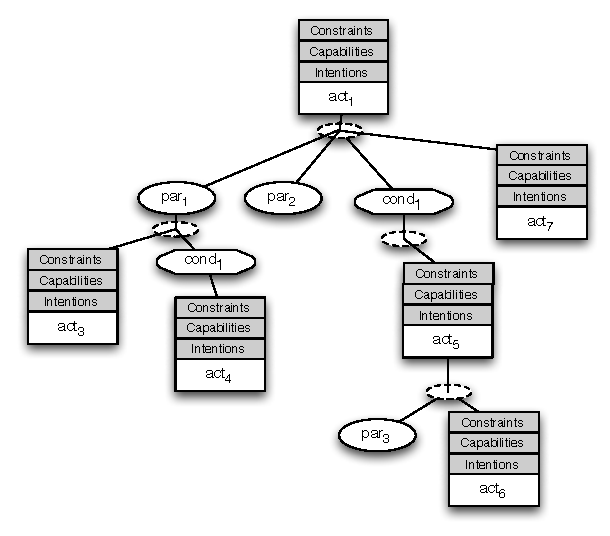
\includegraphics{plangraph.pdf} 
   \caption{Structure of a PlanGraph}
   \label{fig:plangraph}
\end{figure}

\fxwarning {Show a concrete example of plangraph in the motivating scenario}

In many applications, such as the dialog-based interfaces \cite{Cai2003,Cai2005}, the whole collaborative activity can be represented using one single PlanGraph, as the overall goal in one interaction session is unique. However, in complex collaborative activities, it is possible that multiple goals are active at the same time. As a result, the knowledge representation of field of work in these situations is often a forest that includes multiple PlanGraph trees in parallel.
% subsection the_plangraph_model (end)

\subsection{Representing elements and relations} % (fold)
\label{sub:representing_activities}
The PlanGraph model allows us to represent the basic elements and entities in the field of work. The actions, actors, and resources are first-class objects in the PlanGraph model, and the multiple relations among then can be represented as the structural relations in the PlanGraph model (Table \ref{basic_rel_pg}). 

\fxwarning {Add the class diagram or the picture similar to the one used in the social modeling book to show the different entities}

\paragraph*{Actors} % (fold)
\label{par:actors_in_plangraph}
Each actor is represented an object with a unique \emph{ID} in the PlanGraph model. Each actor object in the PlanGraph maintain the current state of the corresponding actor, such as the name, the location, the role of the actor, and the expertise he/she has. Each actor object also maintains a list of actions that the actor is currently participated in.
% paragraph actors_in_plangraph (end)

\paragraph*{Actions} % (fold)
\label{par:actions_in_plangraph}
Actions are modeled as a type of node within the hierarchical structure of the PlanGraph. The \emph{goal} of the action is represented as a condition node, indicating the expected effect of the action when it is successfully performed. The current \emph{execution state} of the action and the \emph{current recipe} to perform this action are stored as attributes of each action node. The \emph{Intentions} and \emph{Capabilities} record the different relations between participating actor towards the action. The \emph{Constraints} record the possible constraint relations between subsidiary actions. The \emph{parameters}, \emph{conditions}, and \emph{sub-actions} point to the other nodes that form the sub-plan of this action.
% paragraph actions_in_plangraph (end)

 \paragraph*{Resources} % (fold)
 \label{par:resources_in_plangraph}
Resources are modeled as parameter nodes in a PlanGraph. Each parameter node records information about the current states of the corresponding resource in the domain, such as the location of a rescue vehicle, or the capacity of the decontamination station. Parameter nodes can be collective or individual. A collective parameter indicates a collection of resources with the same type, for instance, a parameter representing all the victims in the same rescue operation. Each resource points to at least one sub-action that is used to identify the resource, and may points to conditions that the resource needs to satisfy.
% paragraph resources_in_plangraph (end)

\paragraph*{Relations between actors and their actions} % (fold)
\label{par:relations_between_actors_and_their_actions}
The relations between actors and their actions can be directly retrieved from the \emph{Intentions} and \emph{Capabilities} attributes attached to each action, recording the different relations between participating actor towards the action.
% paragraph relations_between_actors_and_their_actions (end)

\paragraph*{Relations between actions} % (fold)
\label{par:relations_between_actions}
The two major types of relations between actions are composition and precedence. The former is directly encoded in the hierarchical structure of a PlanGraph. Each action node has an attribute \emph{sub actions} recording its subsidiary actions under current plan. As a result, the fact that acton $act_1$ is included in the list of \emph{sub actions} of action $act_2$ represents the relation that action $act_1$ is the subsidiary action of doing $act_2$. The precedence relation that reflects the temporal order of doing two actions is encoded in the \emph{constraints} slot of their parent action node.
% paragraph relations_between_actions (end)

\paragraph*{Relations between resources and actions} % (fold)
\label{par:relations_between_resources_and_actions}
The relations between resources and actions are modeled as the composition relations between action nodes and parameter nodes in a PlanGraph. Each action node has a slot \emph{parameters} recording all the parameters under current plan, and each parameter has a slot \emph{sub actions} recording the actions to identify the parameter, and the \emph{conditions} that include subsidiary actions to manipulate the parameter. On the other hand, all the sub actions at the same level of the parameter are consumers of this parameter.
% paragraph relations_between_resources_and_actions (end)

{\footnotesize
\begin{longtable}{>{\raggedright}p{1.5in}>{\raggedright}p{4in}}
\toprule 
Relation & Structure in PlanGraph\tabularnewline
\midrule 
$Pot.Int(ar,act)$ \par $Int.Th(ar,act)$ \par $Int.to(ar,act)$ \par $Perform(ar,act)$ & search the \emph{Intentions} slot attached to each action node: 
\par 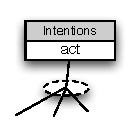
\includegraphics{intentions.pdf}\tabularnewline
\midrule 
$Knows(ar,act)$ \par $Able(ar,act)$ \par $Workable(ar,act)$ & search the \emph{Capability} slot attached to each action node: 
\par 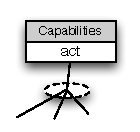
\includegraphics{capabilities.pdf}\tabularnewline
\midrule 
$Sub.Act(act_1, act_2)$ &  $act_1$ is a subsidiary action node under $act_2$: 
\par 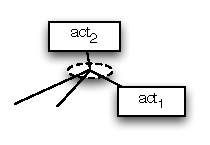
\includegraphics{sub_act.pdf} \tabularnewline
\midrule 
$Precedes(act_1, act_2)$ &  $act_1$ and $act_2$ as ordered siblings: 
\par 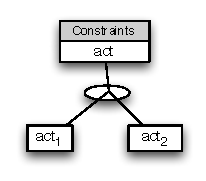
\includegraphics{precedes.pdf}\tabularnewline
\midrule 
$Consume(act, res)$ & a parameter node representing a resource $res$ and  a action node $act$ as siblings: 
\par 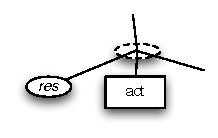
\includegraphics{consumes.pdf}\tabularnewline
\midrule 
$Produces(act, res)$ &  $act$ is a subsidiary action node under the parameter node representing a resource $res$: 
\par 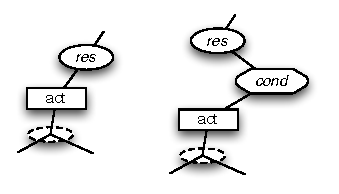
\includegraphics{produces.pdf}\tabularnewline
\bottomrule
\caption{Representing basic relations in PlanGraph}
\label{tab:basic_rel_pg}
\end{longtable}
}
% subsubsection representing_relations (end)
% subsection representing_activities (end)

\subsection{Constructing local scopes} % (fold)
\label{sub:representing_local_scopes}
Based on the definition of local scopes in Section \ref{sub:local_scopes}, the local scope of an actor can be dynamically constructed by depth-first traversing through the PlanGraph model to search for all the actions that have intention or capability relations with the actor.

We define a procedure $BUILD\textrm{-}LS$ that takes an actor object $ar$ and a PlanGraph $PG$ to construct both the local scope of intentions $LSI$ and local scope of capabilities $LSC$ for the actor. We define a sub-procedure $ADD\textrm{-}To\textrm{-}LS$ that takes an actor object $ar$ and a action node $act$ in the PlanGraph to add the action to the local scope $LSI$ or $LSC$ based on whether the corresponding relation exists. The $ADD\textrm{-}TO\textrm{-}LS$ procedure then calls itself on all the children nodes to traverse to the deeper levels in the PlanGraph. In this way, the process to construct the local scopes $BUILD\textrm{-}LS$ is composed of the initialization of $LSI$ or $LSC$, and then a recursive call of $ADD\textrm{-}TO\textrm{-}LS$, beginning on the root node of the PlanGraph.

{\footnotesize
\begin{algorithm}
\begin{algorithmic}[1]
\Procedure{BUILD-LS}{$ar,PG$}
	\State $LSI\gets [\:], LSC\gets [\:]$
	\State $root\gets PG.root$
	\State $ADD\textrm{-}TO\textrm{-}LS(ar, root)$\Comment{start the recursion from $root$}
\EndProcedure
\Procedure{ADD-TO-LS}{$ar,act$}
	\ForAll{$int$ \textbf{in} $act.intentions$}\Comment{check the current node}
   		\If{$int.actor == ar$}
   			\State $LSI.add(ar, act, int)$
   		\EndIf
	\EndFor
	\ForAll{$cap$ \textbf{in} $act.capabilities$}
   		\If{$cap.actor == ar$}
   			\State $LSC.add(ar, act, cap)$
   		\EndIf
	\EndFor
	\ForAll{$par$ \textbf{in} $act.parameters$}\Comment{recursion on parameters}
   		\ForAll{$subact$ \textbf{in} $par.subacts$}
   			\State $ADD\textrm{-}TO\textrm{-}LS(ar, subact)$
		\EndFor
	\EndFor
	\ForAll{$cond$ \textbf{in} $act.conditions$}\Comment{recursion on conditions}
   		\ForAll{$subact$ \textbf{in} $cond.subacts$}
   			\State $ADD\textrm{-}TO\textrm{-}LS(ar, subact)$
		\EndFor
	\EndFor
	\ForAll{$subact$ \textbf{in} $act.subacts$}\Comment{recursion on subacts}
   		\State $ADD\textrm{-}TO\textrm{-}LS(ar, subact)$
	\EndFor
\EndProcedure
\end{algorithmic}
\end{algorithm}
}

If there are multiple actively PlanGraph, the local scopes can be generated by calling $BUILD\textrm{-}LS$ on each PlanGraph, and then merge the local scopes of intentions $LSI$ and local scopes of capabilities $LSC$ separately.

\fxwarning {Show a result of the constructed local scope in the same concrete example of plangraph in the motivating scenario}

% subsection representing_local_scopes (end)

\subsection{Constructing dependency network} % (fold)
\label{sub:representing_dependencies}
From the PlanGraph model, we can also dynamically construct the corresponding dependency network to represent how the actions are dependent on each other. Formally, a dependency network $DN=(V(DN), E(DN), \psi)$ is defined as a directed graph with the following characteristics:
\begin{enumerate}
	\item $V(DN)=\{ACT \cup PARAM \cup COND\}$ is the set of all the nodes in the dependency network, all the \emph{dependers} and \emph{dependees} are action nodes $ACT$, and the \emph{dependums} can be any parameter $RES$ or condition nodes $COND$. 
	\item The set $E(DN)$ is a set of links between the nodes. Each link can be represented as a pair of nodes in $V(DN)$, i.e. $\psi: E(DN) \to V(DN) \times V(DN)$. The link can indicate a direct dependency between two action nodes, or a incoming link that connects a \emph{depender} and \emph{dependum}, or an outgoing link that connects a \emph{dependum} and \emph{dependee}.
\end{enumerate}

The construction of dependency network can be also achieved by depth-first traversing through the PlanGraph model to search for all the action-action and action-resource relations. We define a procedure $BUILD\textrm{-}DN$ that constructs a dependency network from a PlanGraph $PG$. As the set of nodes $V(DN)$ can be calculated from the set of links $E(DN)$ by removing all the duplicate nodes in $E(DN)$. The goal of the $BUILD\textrm{-}DN$ is to build $E(DN)$. Similarly, we define a sub-procedure $ADD\textrm{-}To\textrm{-}DN$ that takes an action node $act$ in the PlanGraph to add dependencies that starting from the node $act$, i.e. the $act$ as the \emph{depender}.

{\footnotesize
\begin{algorithm}
\begin{algorithmic}[1]
\Procedure{BUILD-DN}{$PG$}
	\State $E\gets [\:]$
	\State $root\gets PG.root$
	\State $ADD\textrm{-}TO\textrm{-}DN(root)$\Comment{start the recursion from $root$}
\EndProcedure
\Procedure{ADD-TO-DN}{$act$}
	\ForAll{$subact$ \textbf{in} $act.subacts$}\Comment{check for Sub.Act}
   		\State $E.add(act, subact)$
	\EndFor

	\If{$act.hasParent()$}
		\ForAll{$constr$ \textbf{in} $act.parent.constraints$}\Comment{check for Precedes}
			\If{$constr.next == act$}
   				\State $E.add(act, constr.prev)$ 
   			\EndIf
		\EndFor
		\ForAll{$par$ \textbf{in} $act.parent.parameters$}\Comment{check for parameters}
   			\ForAll{$subact$ \textbf{in} $par.subacts$}
   				\State $E.add(act, par), E.add(par, subact)$
			\EndFor
		\EndFor
		\ForAll{$cond$ \textbf{in} $act.parent.conditions$}\Comment{check for conditions}
   			\ForAll{$subact$ \textbf{in} $cond.subacts$}
   				\State $E.add(act, cond), E.add(cond, subact)$
			\EndFor
		\EndFor
   	\EndIf

	\ForAll{$par$ \textbf{in} $act.parameters$}\Comment{recursion on parameters}
   		\ForAll{$subact$ \textbf{in} $par.subacts$}
   			\State $ADD\textrm{-}TO\textrm{-}DN(subact)$
		\EndFor
	\EndFor
	\ForAll{$cond$ \textbf{in} $act.conditions$}\Comment{recursion on conditions}
   		\ForAll{$subact$ \textbf{in} $cond.subacts$}
   			\State $ADD\textrm{-}TO\textrm{-}DN(subact)$
		\EndFor
	\EndFor
	\ForAll{$subact$ \textbf{in} $act.subacts$}\Comment{recursion on subacts}
   		\State $ADD\textrm{-}TO\textrm{-}DN(subact)$
	\EndFor
\EndProcedure
\end{algorithmic}
\end{algorithm}
}

\fxwarning {Show a result of the constructed dependency network in the same concrete example of plangraph in the motivating scenario}

\fxwarning {should consider the state of the actions here or leave it for belief propagation?}

\fxwarning {how to handle multiple PlanGraphs? shared resource, what else?}
% subsection dependency_relations_in_the_activity_structure (end)
% section representing_the_field_of_work (end)

\section{Representing Events} % (fold)
\label{sec:representing_events}
In Section \ref{ssub:the_concept_of_events}, we discuss the difference between \emph{`occurrence'}, \emph{`awareness'}, and \emph{`event'}, and define \emph{`events'} to refer to the computerized entities that are used in an awareness system to represent knowledge about either real world \emph{`occurrence'} or the results of \emph{`awareness'} processes. Before delving into how events can be used by the computer system to update the knowledge representation of the field of work, or used by the human actors to develop awareness, we need to discuss how they are computationally represented and what types of events are defined in this study. In this section, we first describe the general representational structure of events, then discuss the major types of events, and how they are represented differently.

\subsection{Structure of events} % (fold)
\label{sub:defining_events}
We adopt the similar approach with many existing event processing systems \cite{Mhl2010} to represent each event as a structured object consisting of a named set of attributes. Formally, an event $e$ is a nonempty set of \emph{attributes} $\{a_1, a_2, ..., a_n\}$, where each $a_i$ a name/value pair $(n_i, v_i)$ with name $n_i$ and value $v_i$. It is assumed that names are unique, i.e., $i\ne j \Rightarrow n_i\ne n_j$, and that there exists a function that uniquely maps each $n_i$ to a data type $T_i$ that is the type of the corresponding value $v_i$.

The set of attributes for each event should help answer questions such as this: What occurrence or awareness aspect it refers to? When did it happen? Where did it happen? What other information is associated with its happening? The answers to these questions are usually depend on the type of event they are associated with. An \emph{event type} is a generalization for a set of event objects that have the same semantic intent and same structure \cite{Etzion2010}, i.e. they share the same set of attributes, but may have different values. Each \emph{event type} has a unique event type identifier. In this study we use simple descriptive text strings for these identifiers, for example the phrase \emph{``LocationChanged''} identifies an event type that can describe any instance of an object's location change. Identifying the set of \emph{event types} is an application specific task, as actors in different applications have different awareness needs and capabilities to detect events. We describe the major event types that are supported in this study in Section \ref{sub:event_types}.

As arbitrary attributes can be included in each event type, we can distinguish between three kinds of attributes carried in each event, following the definitions in \cite{Etzion2010} (Figure \ref{fig:event_structure}):

\begin{enumerate}
	\item The \emph{header} consists of generic information about the event, such as the event type and occurrence time, etc. The name and meaning of these header attributes are not specific to a particular event type.
	\item The \emph{payload} contains a collection of attributes carrying the data that describes the actual occurrence. Unlike header attributes independent of the actual event type, the payload attributes are defined per event type. 
	\item An event can also contain free-format \emph{open content} information that provides a mechanism that an event producer or the awareness system can use to enrich an event object with extra contextual information, such as human-readable explanation, multi-media content etc.
\end{enumerate}

\begin{figure}[htbp] %  figure placement: here, top, bottom, or page
   \centering
   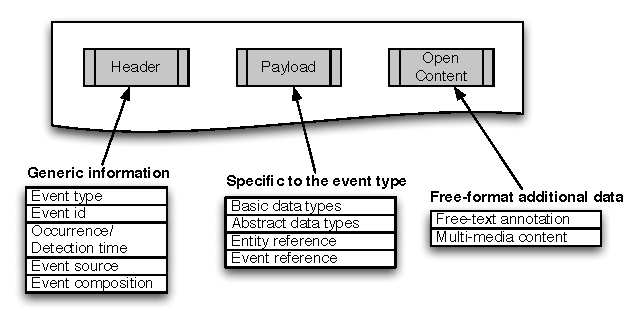
\includegraphics{event_structure.pdf} 
   \caption{The structure of an event (adapted from \cite{Etzion2010} p.63)}
   \label{fig:event_structure}
\end{figure}

\paragraph*{Header} % (fold)
\label{par:header}
The header of an event contains the common attributes that are included in every event object. Unlike payload or open content that are optional, a header is required for every event representation. In general, the header of an event needs to include the following attributes:

\begin{enumerate}
	\item \emph{Event type}. This attributes stores the event type identifier that uniquely identifies the event type of this event.
	\item \emph{Event identifier}. This is a unique identifier for each individual event object.
	\item \emph{Occurrence/detection time}. The occurrence time attribute records the time at which the real world occurrence happens. In some cases, the event producer might not be able to determine the time when the event actually occurred. For example, if the producer examines the state of some external entity only at periodic intervals. In such cases, the detection time is used instead that records the time at which the event became known by the event producer. 
	\item \emph{Event source}. This is the entity that originates this event. This can be either an external sensor, or a human actor in the collaborative system.
	\item \emph{Event composition}. This is a boolean attribute that denotes whether the specific event is a composite event or not. A composite event is one whose payload is made up of several different event instances.
\end{enumerate}
% paragraph header (end)

\paragraph*{Payload} % (fold)
\label{par:payload}
The attributes that make up the event payload are used to carry the data that describes the actual occurrence. The set of attributes included in each event is a variable that depends on the corresponding event type. There are several types of data that can be included as payload attributes:
\begin{enumerate}
	\item \emph{Basic data types}. The value in an payload attribute can simply be in the basic data types, such as string, numeric boolean, date/time etc.
	\item \emph{Abstract data types}. Attributes can also have abstract data types that are structures composed of other data types. For example, many events includes a geographic attribute to records the whereabout of the represented real world occurrence. This attribute can be a point-based representation as a latitude/longitude pair, or more complicated as a route or a geographic area, which are in abstract data types.
	\item \emph{Entity reference}. Instead of records the information directly in an attribute, the event can also records information by pointing to entities represented in the field of work. For example, an \emph{`ActionPerformed'} event may use the reference to the action node stored in the PlanGraph model to indicate which action is performed.
	\item \emph{Event reference}. Some events may contain references to other events. For example, a composite event may use the event references to records the primitive events that it is composed of.
\end{enumerate}
% paragraph payload (end)

\paragraph*{Open content} % (fold)
\label{par:open_content}
The open content of an event can include any attributes an event producer or the awareness system can use to provide additional contextual information about the event. For example, it is used in the awareness externalization process to allow the actors to provide the human-readable explanation of their interpretations.
% paragraph open_content (end)

% subsection defining_events (end)
\subsection{Event types} % (fold)
\label{sub:event_types}
As we argue in Section \ref{ssub:the_concept_of_events} that \emph{events} can be used to represent both description of real world \emph{occurrences} and externalization of human actors' internal \emph{awareness} knowledge, a fundamental distinction should be made between these two categories of events, we call the former \emph{external events}, and the latter {internal events}. The distinction between external events and internal events are important, because (1) they require different representational structures, i.e. the payloads of events have different set of attributes; (2) they are consumed differently by the system when updating the knowledge representation of the field of work; (3) and they are treated differently in  human users' awareness processes. 

Another distinction to make is the difference between \emph{primitive events} and \emph{composite events}. Composite events prevent the users from being overwhelmed by a large number of primitive event by providing them with a higher-level abstraction \cite{Mhl2010}. Generally, a composite event is made up of several other events (either primitive or composite), according to a specification of relations between them. 

In the following, we first describe the major primitive event types in both external and internal categories, and then discuss the composite events as a special event type with its own payload structure.

\subsubsection{External events} % (fold)
\label{ssub:external_events}
As we conceptualize a collaborative environment as consisting of a variety of entities and their relations, the external events can be defined to indicate any kinds of changes on either these entities or their relations. 

\paragraph*{Events on entities} % (fold)
\label{par:events_on_entities_}
We define each external event on an individual entity as a semantic function that changes the entity's property or state. We follow the general event ontology proposed in \cite{Kaneiwa2007} to define the following categories of external events on individual entities:

\begin{enumerate}
	\item \emph{State Change}. An event is a state change event if the occurrence yields a change of states on an entity. All the possible states of an entity are usually can be expressed as a discrete state machine, and each state transition indicates a possible state change event. For example, Figure \ref{fig:action_exec_state_trans} shows the transition diagram with all the possible execution states of an action. Each valid transition in the diagram can be considered as a state change event.
	\begin{figure}[htbp] %  figure placement: here, top, bottom, or page
   	\centering
   	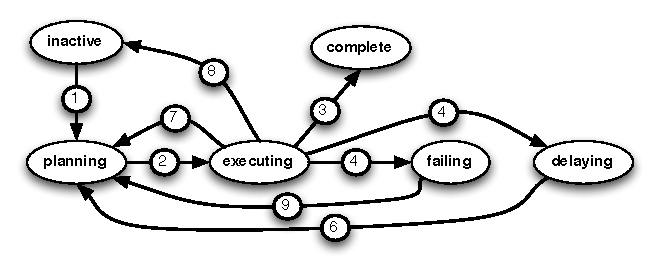
\includegraphics{action_exec_state_trans.pdf} 
   	\caption{Execution state transition of an action}
   	\label{fig:action_exec_state_trans}
	\end{figure}
	\item \emph{Existential Change over Time}. An event indicates an existential change over time if its occurrence changes the existence of an entity in temporal order, e.g. an entity did not exist in the past but it exists now.
	\item \emph{Existential Change over Space}. An event indicates an existential change over space if its occurrence changes the existence of an entity depending on its movement through space, e.g. an entity existed at location A, but now exists at location B. 
	\item \emph{Value Comparison}. Another common class of external events are comparison events to indicate changes on attribute values of an entity. They can used to indicate whether an attribute value is equal, unequal, greater than, or less than a fixed threshold, or the same attribute value in the past. 
\end{enumerate}
% paragraph events_on_entities_ (end)

\paragraph*{Events on relations} % (fold)
\label{par:events_on_relations}
The events on relations are used to indicate whether some relations between entities hold. For example, an event with the type \emph{`ResourceAssigned'} indicates an assignment relation between a resource and an action starts to hold, i.e. the resource is now assigned for performing the action. Therefore, the types of external events on relations depend on the possible types of relations that can be identified in the domain. 

Generally, the basic relations between entities in the real world can be divided into three categories: spatial, temporal, and conceptual \cite{Tomaszewski2010}.

\begin{enumerate}
	\item The spatial relations link the entities through their spatial positions. The basic types of spatial relations have been well studies in the literature on geographic information systems, include binary topological \cite{egenhofer1994deriving}, directional \cite{frank1991qualitative}, and distance relations \cite{hernandez1995qualitative}. Topological relations is a particular subset of geometric relations that are preserved under topological transformations such as translation, rotation, and scaling. Some examples are relations indicating whether one entity disjoints, meets, overlaps, or contains another entity. Directional relations indicate the relative direction between two entities, such as one is at north of the other. Distance relations link entities based on their proximity in the space, such as one is within a certain range of another. 
	\item The temporal relations link the entities based on their temporal positions. The basic types of temporal relations are considered in the literature on temporal reasoning \cite{allen1994actions}, including binary topological, ordering, and distance relations \cite{Andrienko2011}.
	\item The conceptual relations are an umbrella term that cover all the different types of organizational, structural, or social relations between entities in a particular collaborative activity. 
\end{enumerate}

From the basic types of relations, more complex types of relations can be built, such as
density (clustering, dispersion), arrangement (e.g. sequence in time or alignment in space) and spatial-temporal relations. The latter are composed of spatial and temporal relations and represent changes of spatial relations over time: approaching or going away, entering or exiting, following, keeping distance, concentrating or dissipating and so on.
% paragraph events_on_relations (end)

Figure \ref{fig:external_events} shows an upper level typology of the external events that can be defined on entities and relations in a collaborative environment.
\begin{figure}[htbp] %  figure placement: here, top, bottom, or page
	\centering
	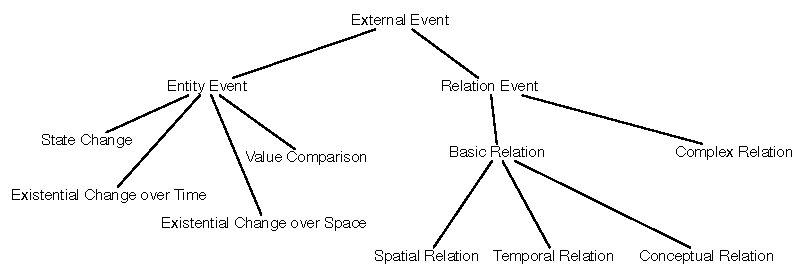
\includegraphics{external_events.pdf} 
	\caption{An upper level typology of external events}
	\label{fig:external_events}
\end{figure}

\paragraph*{Relevance to the field of work} % (fold)
\label{par:relevance_to_the_field_of_work}
 Although the number of external events that could be possibly identified is infinite, not all of them are relevant to the human actors' working context, i.e. the field of work. As a result, our goal of identifying external events focuses on finding a subset of event types that are relevant in an application domain. Existing studies to identify such a subset of event types are usually done in two ways \cite{Pottebaum2011}: from the `supply' side to identify the set of event types that can be recognized by available sensors, and from the `demand' side to define event types based on the nature of the activities supported by the event-based systems. As we are more concerned about the human actors' awareness needs in performing their collaborative activities, we follow the `demand'-side approach and identify the major event types based on how they could possibly contribute to the understanding of the field of work in a collaborative activity. 

 In general, we believe that the relevance of external events to the field of work can be analyzed based on the different functional roles they can play in updating the knowledge about the field of work. If the occurrence of an external event can imply some change in the field of work, it should be treated as relevant. Based on our conceptualization of the field of work, we can identify the following function roles for external events:

 \begin{enumerate}
 	\item \emph{Direct change to entities in the field of work}. The external events can indicate changes on individual entities that are modeled in the field of work, i.e. the property or state change on the resources, actors, or actions. For example, a state change event can be used to indicate the change of execution state for an action in the field of work. Location change events can be used to describe an actor's movement in the field of work. 
 	\item \emph{Direct change to relations in the field of work}. Within the different types of relation events that can be possibly identified, some of them are directly related to the various relations between resource, actors, and actions as we described in Section \ref{ssub:relations}. For example, an external event type indicating the constitution relation between two entities can be used to describe the $Sub.Act$ relation between two actions, i.e. one action is a subsidiary action to perform another one. The assignment relation event types can be used to describe relations between an actions and a resource, i.e. the resource has been assigned to the performance of the action. 
 	\item \emph{Action motivation}. Aside from the two cases that external events can be directly linked to the entities and relations in the field of work, the external events can also impact the field of work by motivating the actions that need to be performed. For example, an external event indicating that the fire alarm is ringing will activate my goal to escape from my office. In this case, the fire alarm is not directly linked to any entities in my current field of work, rather it motivates me to perform a new action.
 	\item \emph{Indication of action performance}. In some cases, the external events can also provide some evidence implying the effects of action performance. For example, instead of a state change event directly showing the action to delivery a resource to an actor has been completed, it could be implicitly inferred from a spatial relation event that indicates the resource is now located at the actor's location. Similarly, an external event indicating the occurrence of a traffic blocking between the resource's current location and the actor's implies the delivery action is delayed.
 \end{enumerate}
% paragraph relevance_to_the_field_of_work (end)
% subsubsection external_events (end)
\subsubsection{Internal events} % (fold)
\label{ssub:internal_events}
The internal events are used to describe the results of human actors' awareness processes. Unlike the external events can describe any entities and relations in the real world, they describe the changes of human actors' internal mental states in the field of work. The internal events are usually derived from the external events to indicate the human actors' interpretation on these external events. In this study, we identify two types of internal events: \emph{intention} events and \emph{belief} events. 

An \emph{intention} event indicates a human actor's adoption of certain intention towards some action in the field of work. As we described in Section \ref{ssub:relations}, an actor's intention to an action can be of different kinds, i.e. $Pot.Int$, $Int.Th$, or $Int.To$, with  different levels of commitment. Figure \ref{fig:intention_event} shows the basic structure of an intention event. The payload of an intention event include three required attributes: an intention type indicating whether it's a potential intention, intention-that, or intention-to, a reference to the actor entity who has this intention, and a reference to the action that is intended to. An optional free-text attribute is included in the open content part of an intention event, where the human actor can provide the rationale for adopting the corresponding intention.
\begin{figure}[htbp] %  figure placement: here, top, bottom, or page
	\centering
	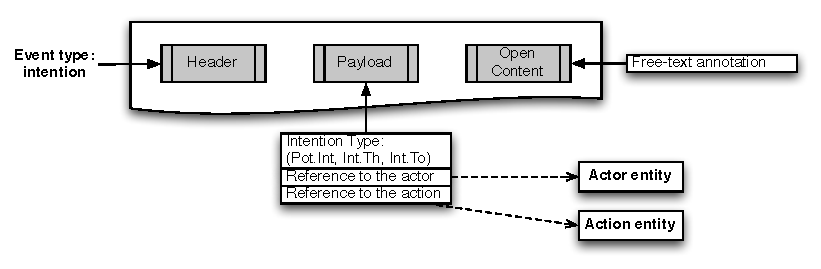
\includegraphics{intention_event.pdf} 
	\caption{Structure of an intention event}
	\label{fig:intention_event}
\end{figure}

An \emph{belief} event describes a belief of a human actor on some occurrence in the field of work. For example, it can be used to indicate an actor's belief that an action has been successfully performed, or his/her belief that he/she has the capability to perform an action. As belief events usually refers to some occurrence in the field of work, we represent belief events by embedding an external event representing the occurrence into its payload (Figure \ref{fig:belief_event}). However, unlike the standalone external event that indicates changes already happened, the occurrence described in a belief event can be something that will happen in the future. These belief events represent the results of the human actor's projection process, i.e. what he/she expects to happen in the future. There are two attributes in a belief event's open content part: the free-text explanation of this belief, and a confidence level to describe how confident he/she is about this belief.
\begin{figure}[htbp] %  figure placement: here, top, bottom, or page
	\centering
	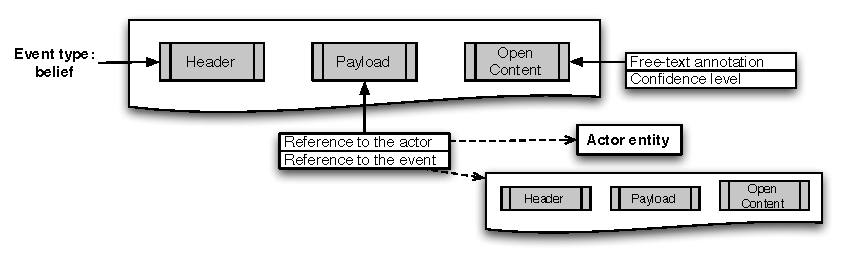
\includegraphics{belief_event.pdf} 
	\caption{Structure of a belief event}
	\label{fig:belief_event}
\end{figure}
% subsubsection internal_events (end)

\subsubsection{Composite events} % (fold)
\label{ssub:composite_events}
Composite events are a special type of events that can consist of several other events. The subsidiary events can be external or internal. Besides the list of subsidiary events, a composite event needs to also describe how these sub-events are combined together. In a simplest case, a composite event can occur only when all the sub-events occur. Moreover, a composite event can occur when some of the sub-events occur, but some do not. Or it occurs when any of the sub-events occur. A more complicated composite event language can be found in \cite{Mhl2010} that includes different relations between the sub-events, such as negation, concatenation, sequence, iteration etc. To describe the composition pattern, a specific payload attribute needs to be included in a composite event's representation (Figure \ref{fig:composite_event}).
\begin{figure}[htbp] %  figure placement: here, top, bottom, or page
	\centering
	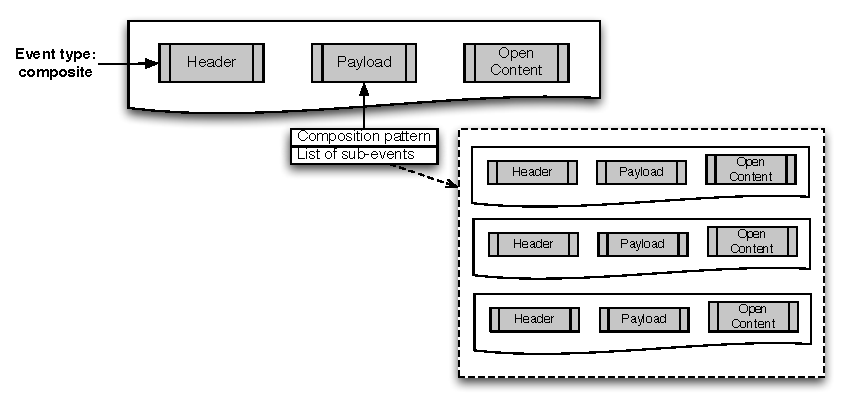
\includegraphics{composite_event.pdf} 
	\caption{Structure of a composite event}
	\label{fig:composite_event}
\end{figure}
% subsubsection composite_events (end)
% subsection event_types (end)
% section representing_events (end)

\section{Discussion} % (fold)
\label{sec:knowledge_representation_discussion}
In this chapter, we first focus on the knowledge representation of the field of work. We employ the PlanGraph model to represent the basic entities and relations in the field of work, and then use this model to derive the knowledge about local scopes of work and dependencies. The PlanGraph theory exhibits some important characteristics that make it suitable to satisfy the three requirements for representing the field of work described in Section \ref{sub:computational_representation_of_the_field_of_work}.

\begin{enumerate}
   \item The PlanGraph models collaborative activities as hierarchically structured subsidiary actions. The basic components of actions, parameters, conditions, and contraints can be used to capture all the basic activity entities and the relations between them can be used to derive the various dependency relationships. 
   \item The PlanGraph model also encodes the mental attitudes requirements of human actors in the actions, including different types of intentions and beliefs on their capabilities. This knowledge provides the basis to identify local scopes of participants. 
   \item A critical point made in the PlanGraph model is the emphasis on the development of collaborative activities. With the development of the activity, the PlanGraph model needs to be updated accordingly, so that it always models the current state of the field of work. 
   \item The PlanGraph model provides a set of reasoning capabilities that can be operationalized to support computer reasoning.  
\end{enumerate}

In this chapter, we have demonstrated the first two characteristics of the PlanGraph model, but leave the knowledge updating and reasoning capabilities to the next few chapters.

Following that, we discuss the representation of events and identify the major events supported in this study. The central idea of our approach is the interaction between these two knowledge components. On one hand, the various events are consumed by the computer system to update its PlanGraph-based representation of the field of work (Chapter \ref{cha:knowledge_updating}). On the other hand, the PlanGraph model enrich the events with more meaningful contextual information, which is then used in the event-driven awareness processes (Chapter \ref{cha:mediate_individual_awareness_processes}). 
% section knowledge_representation_discussion (end)
% chapter knowledge_reprsentation (end)




 

